\chapter{Nerve cells (neurons)'s component}
\label{sec:nerve-cells}

In the early days, it was not know whether the tissues in the brain are composed
of cells. Many believed that all neurons are not separated entity, but were
connected to form one enormous synytium. At the end of 19th century, Ramon y
Cajal showed that each neuron is a closed unit and that each unit interacts with
each other at specialized contacts called synapses. However, the detail
structure of synapses were not know until recently, using electron-microscopic
(EM).

\begin{figure}[htb]
\centerline{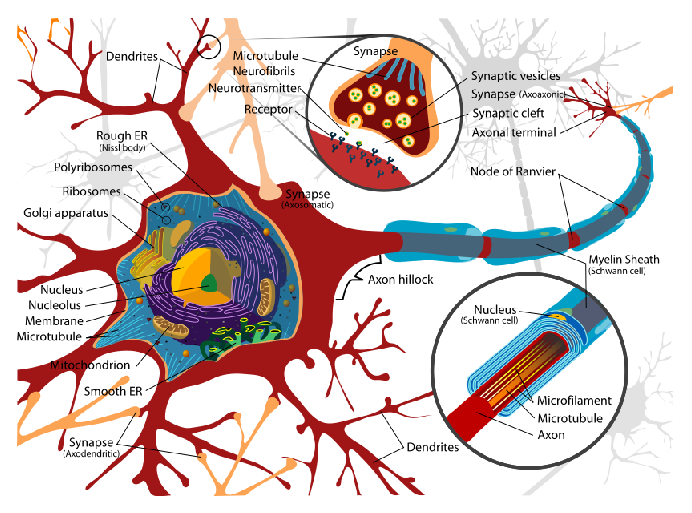
\includegraphics[height=8cm]{./images/Complete_neuron_cell_diagram.eps}}
\caption{A typical Type I nerve cell with supporting glial cells}\label{fig:neuron}
\end{figure} 


{\bf Nerve cells} (neurons): The central to the CNS is nerve cells which belong
to the class of {\it excitable cells}, i.e. it can receive the stimulus and fire
a stimulus to other cells.
The transmission on the dendrite is passive (short distance), while that in the
axon is active (long distance and requires amplification of the signal at the
myelinated sheaths).
In early days of neuroscience, they only able to study the axon of the nerve
cell due to its large size. \citep{hodgkin1948} 


The structure of a nerve cell (aka {\it neuron}) which may come in different
shapes and sizes. The different cell types is disscussed in
Sect.\ref{sec:neuron-types}. In this section, we discuss different components in
a nerve cell.

\section{Components}

A typical neuron consist of 3 parts: dendrites (Sect.\ref{sec:dendrites}), soma
(body - Sect.\ref{sec:Soma}) and the axon (Sect.\ref{sec:Axon}), as shown in
Fig.~\ref{fig:neuron_cell}. \textcolor{red}{A nerve cell has maximum one axon,
but can have many dendrites} (Sect.\ref{sec:neuron-types}). Each branch
(dendrite, axon) is called {\bf a process}.

The part of the axon adjacent to the soma is the axon hillock
(Sect.\ref{sec:axon-hillock}). The axon can branch into several {\bf
telodendria}


there are branches of synapses (Sect.\ref{sec:synapse}). A neuron
may receive input along its dendrites from a number of neurons, via the synapses ({\bf convergence}),
reaching the soma, and then transmit a signal along its axon to many other
neurons, via the synapses ({\bf divergence}) as well. The behavior of the
dendrites, axon, and synapses are all quite different.

% \begin{figure}[hbt]
%   \centerline{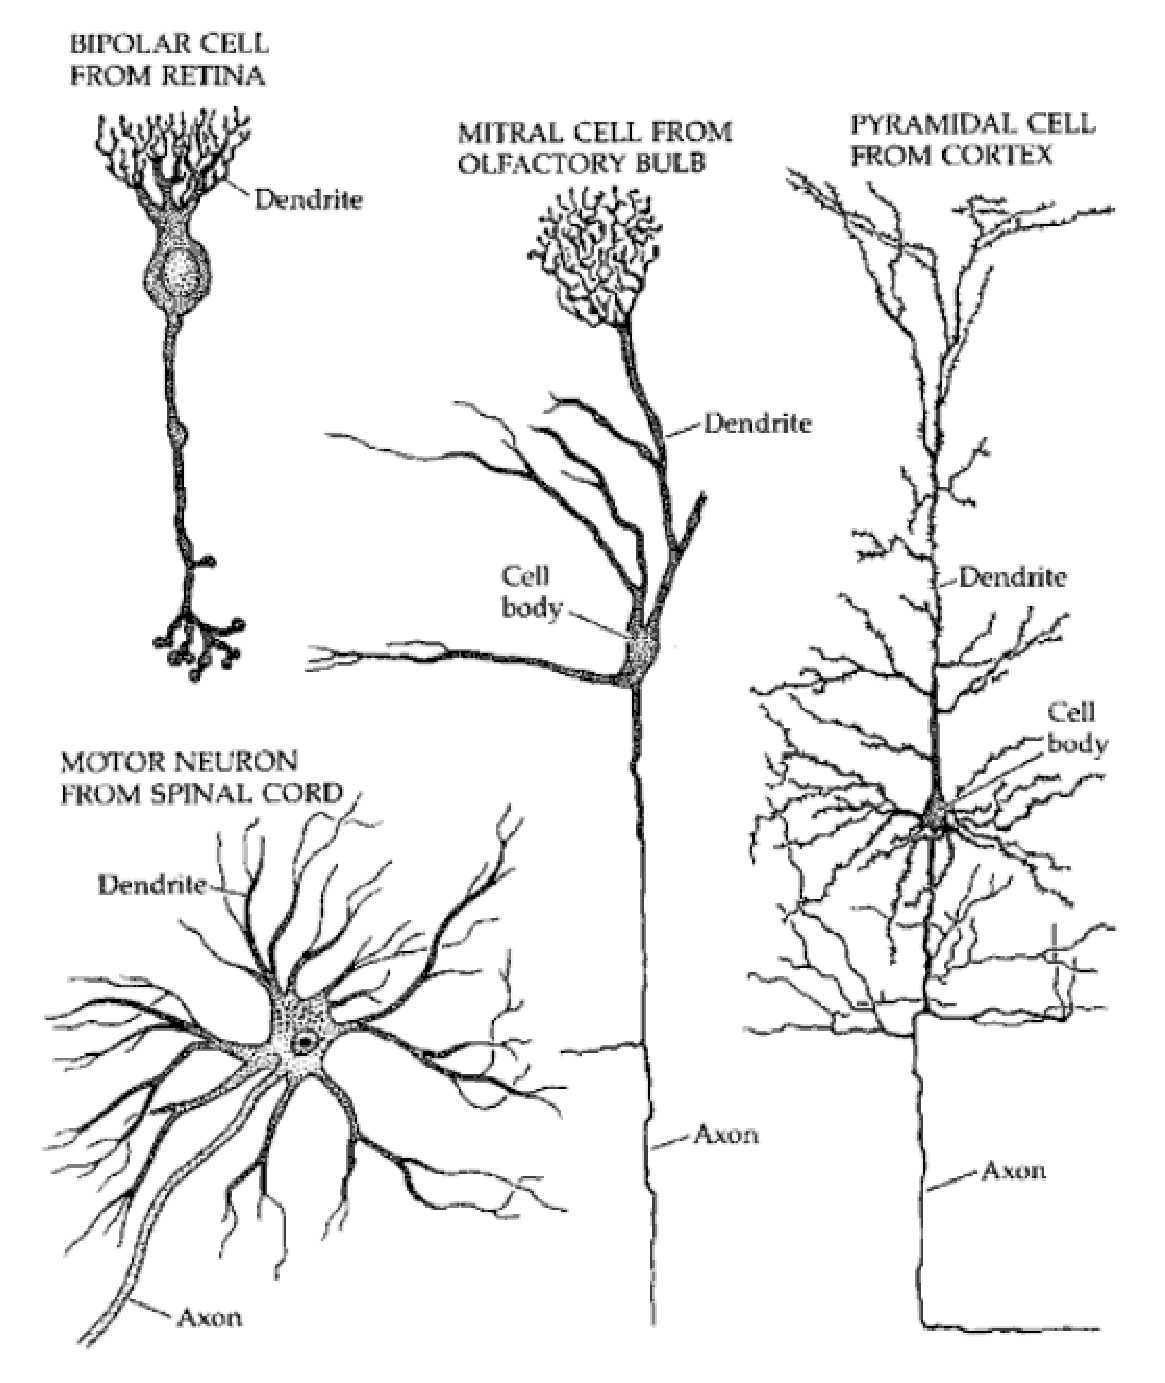
\includegraphics[height=8cm,
%     angle=0]{./images/neurons.eps}}
% \caption{Different morphologies of neurons}
% \label{fig:neurons}
% \end{figure}
\subsection{Axon vs. Dendrite morphology}

{\bf Why do dendrites narrow while axons maintain a constant diameter?}
\footnote{\url{https://www.quora.com/Why-do-dendrites-narrow-while-axons-maintain-a-constant-diameter}}
\begin{enumerate}
  
  \item  Two unique aspects of an axon are that they often travel long distances
  (1 centimeter to 1 meter), and that their job is to carry an all-or-nothing
  pulse signal (the spike) the full distance of the axon via local repeaters
  that keep the signal from decaying. Thus the axon functions primarily as a
  binary signal transmission cable, branching only at the end.
  
  \item The dendrites, in contrast, are local and tend to be a branching tree
  shape only 1mm or so across. Their job is to accurately add up very tiny electrical signals from their inputs.
   The dendritic tree is like an electrical river with tributaries that collect
   and aggregate signals.
  
  The thicker diameter dendrites at the base need to physiologically support the
  full tree structure, whereas the thin tips need only collect minute electrical signals.
  
  
\end{enumerate}

\subsection{How dendrite grows?}

Because of the wide variety of neurons in the human brain, the pattern of
growth will vary between the different types. A pyramidal cell in the cerebral
cortex will have different arborization (branching) patterns than a cerebellar
purkinje cell.
\url{https://www.quora.com/How-do-dendrites-grow}

The morphogenesis of dendritic trees is regulated by innate genetic factors,
neuronal activity, and external molecular cues (Libersat and Duch 2004;
McAllister 2000; Miller and Kaplan 2003; Wong and Gosh 2002) during
developmental and experience-dependent plasticity (Spitzer 2002; Wong and Wong
2000). Furthermore, alterations in neural morphology may occur during aging and
neurodegenerative diseases (De Brabander et al. 1998; Uylings et al. 2000) -
\citep{evers2004}.


Dendrites will grow on their own even if they are isolated from other neurons.
This suggests that neurons are genetically predisposed to grow even without
environmental input. Similarly, \citep{memelli2013} suggested self-referential
force is enough to explain the growth. 

\begin{enumerate}
  \item dendrite growth is dependent on calcium: via (1) BDNF, and (2) by
  activating the cytoskeleton in dendrites
  
  An influx of calcium can can activate CaMKIV, a kinase that activates
  transcription factors, i.e. BDNF (Sect.\ref{sec:BDNF})
  
  The very tip of a dendrite( or an axon) is called a "growth cone", the area
  where the end is elongating.
  The mechanism by which a dendrite and an axon grow is quite similar. Once
  the cytoskeleton has been activated by calcium, it "pushes" against the
  membrane of the dendrite. Small "filopedia" start to form, increasing the
  length of the dendrite.
  
  \item 
\end{enumerate}

\subsection{- role of Golgi apparatus}

Altering the orientation of the Golgi apparatus in hippocampal neurons, which is
constituted by a perinuclear organelle
orientedtowardstheapicaldendriteandadditionalsatellite structures distributed
throughout the dendritic arbor (Golgi outposts), differentially limits dendritic
growth.

Recent studies have begun to elucidate the function of satellite Golgi outposts
and endosomes in polarized neuronal trafficking.

\subsection{- role of ER}

ER (Sect.\ref{chap:ER})

\section{Dendrites}
\label{sec:dendrites}

As shown in Fig.~\ref{fig:neuron}, {\it Dendrite} (Greek, {\it tree}) is a
branch from the soma that receives the signals from other neurons and conducts the
received stimulus (electrochemical signal) to the cell's soma. 
Dendrites differ from axons in many important respects, both morphologically and
functionally. 
\begin{itemize}
  \item Unlike axons, dendrites have tapering processes such that distal
  branches have smaller diameters than proximal ones.
  
  \item Dendrites have specialized structures including spines, which are the
  main excitatory synaptic sites that are not found in axons.
  
  \item  Golgi outposts, found primarily in dendrites.
  
  \item The orientation of microtubules also differs considerably in dendrites
  and axons; in both vertebrates and invertebrates, the microtubules uniformly
  orient with their plus-end distally in axons, whereas dendrites contain
  microtubules of both orientations.
  
\end{itemize}

Dendrites of neuron have been considered as a {\it passive transmitter}, i.e. 
dendrite cannot transmit the signal in a far distance due to the decay of the
electrical signal via leakage current.
However, recent studies have showed that there are voltage-gated ion channels on
the dendrite, i.e. active conductances. In pyramidal layer 5 neurons, the
apical dendrites have $\Na$ channel, $\Ca$ channel, and also $\K$ channels.

There are a large number of dendrites in a nerve cell, and the signal will be
summed at the soma from the stimulus from all dendrites. Such signal will then
be transmitted to other neurons via the axon.

In terms of dendritic arborization, there are 4 classes \citep{yuh-nung2010}:
\begin{enumerate}
  \item class I : 
  
  class I dendritic arborization neurons extend secondary dendrites mostly to
  one side of the primary dendrite.
  
  \item class II:
  
  class II dendritic arborization neurons have more symmetrically bifurcating
  dendrites.
  
  \item class III:
  
  class III dendritic arborization neurons have larger fields and greater
  branching complexity, plus the distinguishing feature of numerous spiked
  protrusions (dendritic spikes) that are rich in actin and lack stable
  microtubules.
  
  \item class IV:
  
   Class IV dendritic arborization neurons are the most complex in branching
   pattern (although they lack dendritic spikes) and achieve nearly complete
   coverage of the body wall.
   
\end{enumerate}

Many factors shape the morphology of a dendritc arbor, including
transcription factors, regulators of microtubules and actins (the primary
cytoskeletal elements for major dendritic branches and terminal dendritic
branches, respectively), Golgi outposts and signalling molecules such as Hippo
and Tricornered (TRC) that mediate dendrite-dendrite interactions.

\subsection{Dendritic branching (dendritic arborization)}
\label{sec:dendritic-branching}

Dendritic branching is also called "dendritic arborization" and "dendritic
ramification."


\subsection{Dendritic shafts}
\label{sec:dendritic-shaft}

{\bf Dendritic shafts} refer to the main body fo the dendrite;
while the dendritic spine (Sect.\ref{sec:dendritic_spines})
is separated from the shaft by a dendritic neck that is often thin ($< 0.6\mum$
and up to a few micrometers in length). 

\subsection{-- tufted dendrite}
\label{sec:tufted-dendrite}

This is not a diferent dendrite, but is just named to considered the region of
the dendrite at the terminal end in pyramidal neurons Layer 5, i.e. the part
about 800 $\mum$ apart from the soma. This part in PL5 typically receives lots
of inputs.

\section{Dendritic spines}
\label{sec:dendritic_spines}

{\bf Dendritic spines} are small branches stemming from the dendrites and form
the synapse with an axon terminal from another neuron. Spines typically receive
{\it excitatory} inputs from a single synapse of axon (Sect.\ref{sec:synapse}),
Fig.\ref{fig:dendritic_spines}; though sometimes both inhibitory and excitatory
connections are made onto the same spine head.

Spines are found on most principal neurons which receives glutamatergic inputs:
\begin{itemize}
  \item pyramidal neurons of neocortex - Sect.\ref{sec:pyramidal-neurons}
  \item medium spiny neurons of striatum - Sect.\ref{sec:medium_spiny_neurons}
  \item Purkinje cells of cerebellum - Sect.\ref{sec:Purkinjie_nerves}
\end{itemize}
Modeling dendritic spines is discussed in Sect.\ref{sec:dendritic_spines_model}.

\subsection{Geometry}
\label{sec:spine-geometry}

The detailed structure of a dendritic spine is given in
Fig.\ref{fig:dendritic_spines_mushroom}. A dendritic spine  has two parts:
{\it spine head} and {\it spine neck}.
\textcolor{red}{However, spine morphology is not static but very 'plastic';
spines change size and shape and numbers over variable timescales} \citep{hering2001}
(within seconds to minutes due to actin remodeling -
Sect.\ref{sec:actin_remodeling}).

Smith et al. (2009) showed morphological differences and regulatory changes
induced by dopamine depletion on glutamatergic transmission at axo-spinous
synapses established by cortical versus thalamic inputs to the striatum.


\subsection{-- Spine head}
\label{sec:spine-head}

shape: thin, stubby, mushroom- and cup-shaped (branched)
   \begin{itemize}
     \item {\bf thin spine} = has long neck
     
     \item {\bf mushroom spine} = has big head
     
     \item {\bf stubby spine}
     
     \item {\bf cup-shaped spine} = 
   \end{itemize}
The variable spine shape and volume is thought to be correlated with the
strength and maturity of each spine-synapse.

As the change in $[\Ca]$ in the spine is not always reflected in $[\Ca]_s$
synapse, it indicated that the spine may contain an independent
calcium-regulating mechanisms \citep{segal2002}. Each spine contains 1-20
voltage-sensitive calcium channel.

As there are also several different types of calcium-permeable receptor/channel
that are colocalized in spines, the spine head can act as an efficient
integrator of different postsynaptic signals. 
However, the physiological significance of
spines for brain function is still not clear.

Ion channels on spines
\begin{itemize}
  \item Glutamate receptors (GluRs): NMDA glutamate receptor
  (NMDAR) and AMPA glutamate receptor (AMPAR) - Sect.\ref{sec:glutamate_receptor}
  
GluRs is anchored to the membrane by cytoskeletal element, at a region called
{\bf postsynaptic density} (PSD) - an electrondense region at the tip of the
spine (10\% of the spine's membrane surface area) and directly appose the active
zone of its synapsing axon. Neurotransmitters released from the active zone bind
receptors in the postsynaptic density of the spine.
Signaling from GluRs is mediated by the presence of an abundance of proteins,
especially kinases, that are localized to the postsynaptic density:
\begin{itemize}
  \item CaMKII - Sect.\ref{sec:CaMKII}
  \item PKC 
  \item PKA - Sect.\ref{sec:PKA}
  \item PP-1 (Protein Phosphatase-1)
  \item Fyn tyrosine kinase
\end{itemize}
 
  \item TrkB receptor for BDNF: play a role in spine survival
  (Sect.\ref{sec:BDNF})
  
  \item Cadherin: forms cell-to-cell junctions between the two neurons.
  
1/2 of the synapsing axons and dendritic spines are physically tethered by
$\Ca$-dependent cadherin.
\end{itemize}
   
\subsection{-- Spine neck}
\label{sec:spine-neck}

spine neck: $0.5-2.0\mum$, even up to 6$\mum$ in CA3 subfield of
  hippocampus
   
volume (variety of sizes): from less than 0.01 $\mum^3$ to
   0.8$\mu^3$ [NOTE: 1$\mum^3$ = $10^{-3}$pL]
   

Compartmentalization via spines allows the changes in the state of an individual
synapse without necessarily affecting the state of other synapses of the same neuron.
The length and width of the spine neck has a large effect on the degree of
compartmentalization, with thin spines being the most biochemically isolated spines.

\subsection{Density}

\textcolor{red}{DENSITY}: Dendritic spines occur at a density of up to 5
spines/1 $\mum$ stretch of dendrite.
 \textcolor{red}{The dendrites of a single neuron can contain hundreds to
thousands of spines}.
It serves as a storage for synaptic strength that help transmit electrical
signals to the neuron's cell body (to be explained shortly).

\subsection{Functional role}

The role of dendritic spines as the contacting sites between neurons was first
described by Santiago Ramon y Cajal on cerebellar neurons at the end of 19th
century. This was first experimentally confirmed via electron microscopy in 
1959 by Gray \citep{gray1959}. It was first believed that dendritic spines does
not change, i.e. remain stable after birth. Interestingly, new techniques of 
confocal microscopy demonstrated that dendritic spines are indeed motile and
dynamic structures that undergo a constant turnover, even after birth
\citep{dailey1996, bonhoeffer2002, yoshihara2009}. 

\begin{figure}[htb]
\centerline{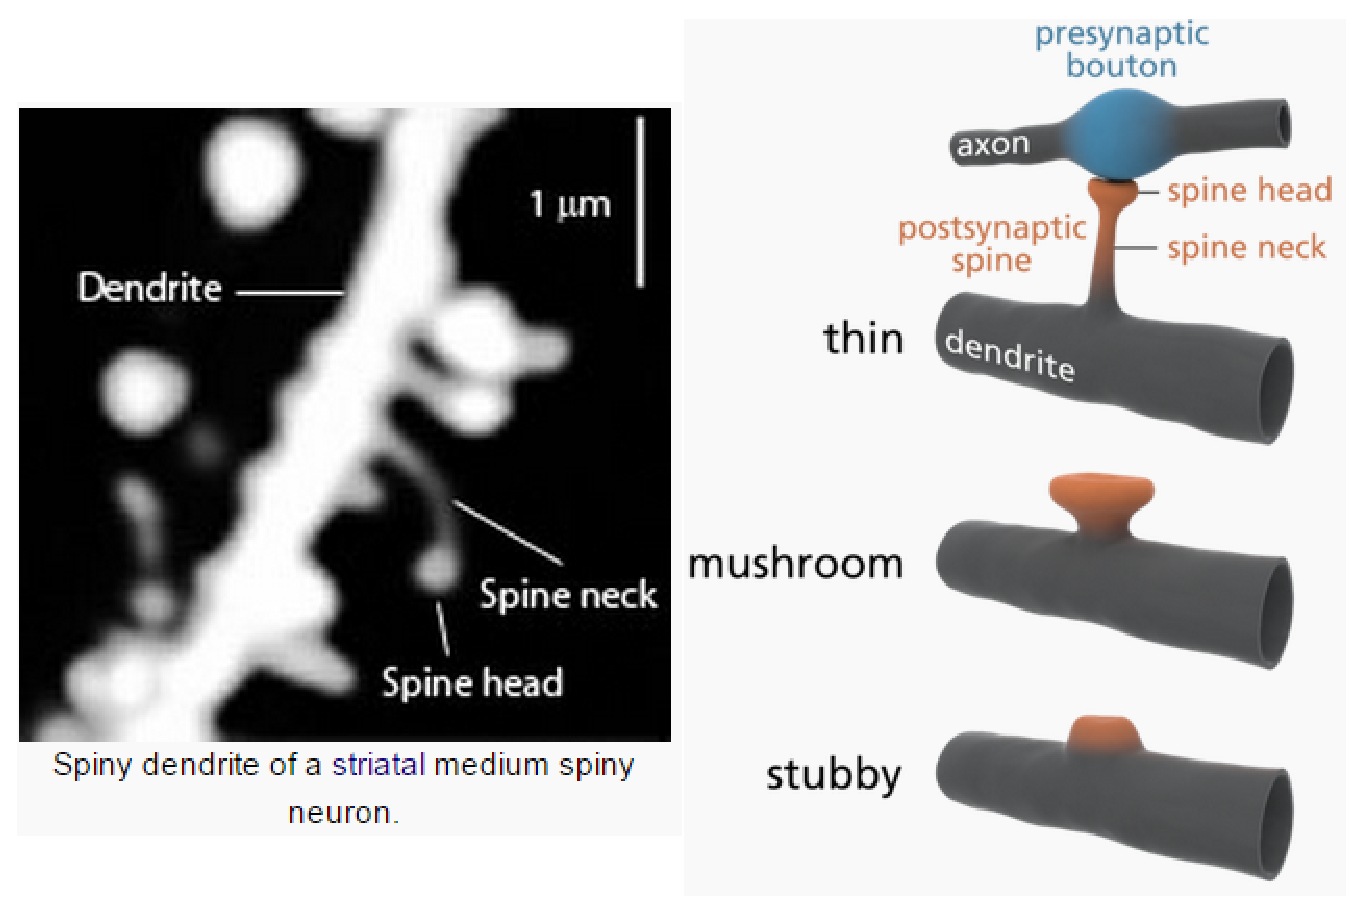
\includegraphics[height=7cm]{./images/dendritic_spines.eps}}
\caption{Dendritic spines in the striatal medium
spine neurons
(Sect.\ref{sec:medium_spiny_neurons}). (B)
Different types of dendritic spines: thin,
mushroom, and stubby}\label{fig:dendritic_spines}
\end{figure} 


Dendritic spines are major sites of excitatory synapses in the brain and display
rapid motility, which is believed to be important for synapse formation and
plasticity (Sect.\ref{sec:synaptic_plasticity}). It is considered as the
elementary structural unit of synaptic plasticity \citep{segal2002}. It has been
suggested that there are two forms of spine mortility \citep{tashiro2004}.  

\begin{figure}[htb]
\centerline{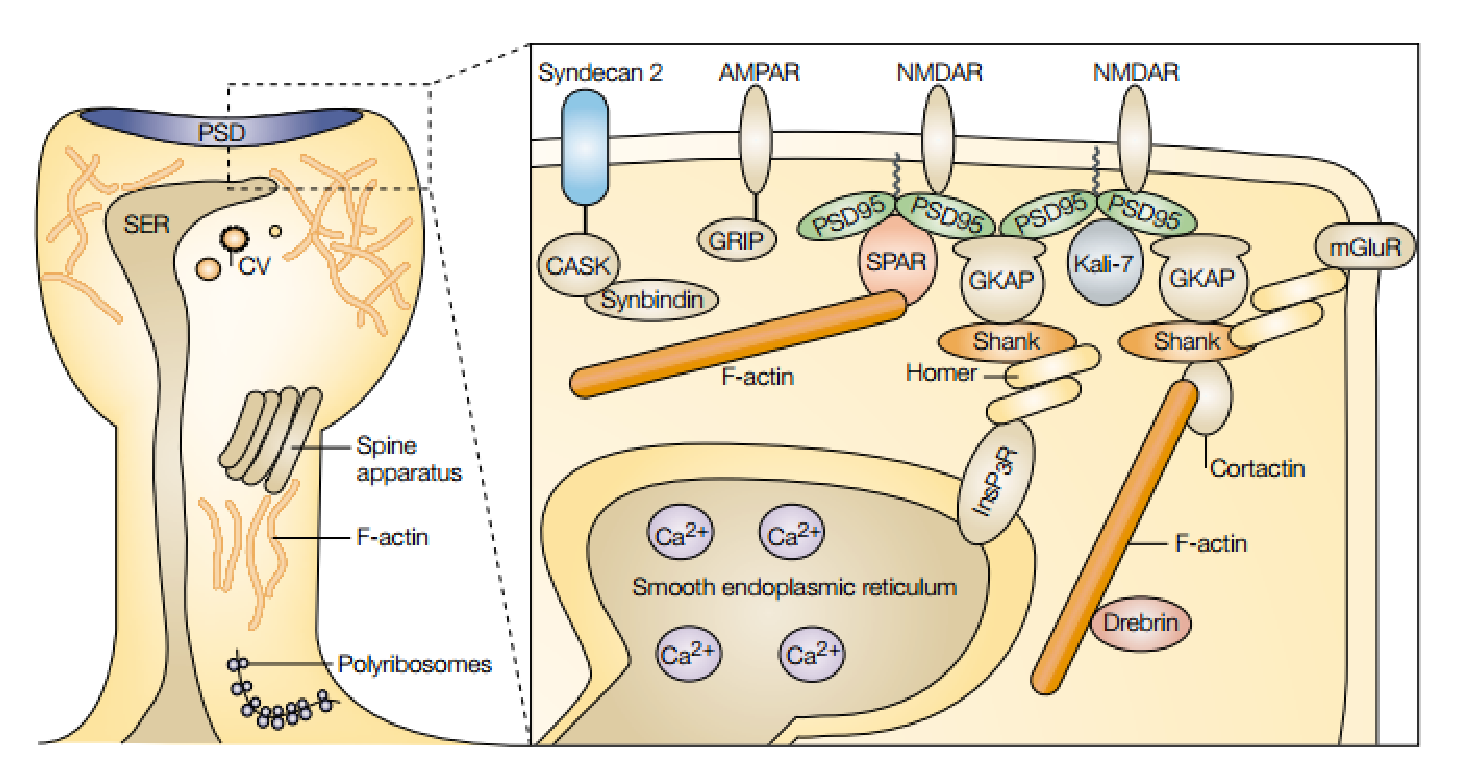
\includegraphics[height=7cm]{./images/dendritic_spine_mushroom.eps}}
\caption{The detailed structure of a mushroom-shaped dendritic spine}
\label{fig:dendritic_spines_mushroom}
\end{figure} 



\subsection{Smooth ER (SER) or spine apparatus (SA)}
\label{sec:Smooth-ER}

Spine apparatus (SA) or smooth ER is a specialized form of endoplasmic reticulum
(ER) that is found in a subpopulation of dendritic spines in central neurons.
Smooth endoplasmic reticulum (SER) is important for regulating calcium which has
been shown to be present at high levels in activated dendritic spines.
SER in the dendrite is contiguous with the SER entering the thin neck of a large
dendritic spine.

The actin binding protein synaptopodin is an essential component for forming
SER.
Mice that lack the gene for synaptopodin do not form a SER.
The SA is believed to play a critical role in learning and memory, but the exact
function of the spine apparatus is still considered relatively enigmatic.

\url{https://en.wikipedia.org/wiki/Spine_apparatus}

\url{http://synapses.clm.utexas.edu/anatomy/images/webserpage.stm} 
\section{Soma}
\label{sec:Soma}

As shown in Fig.~\ref{fig:neuron}, {\it Soma} is the nerve cell's body.

\section{Axon}
\label{sec:Axon}

As shown in Fig.~\ref{fig:neuron}, {\it Axon} (nerve fiber) is a long, slender
projection of nerve cells stemming from the soma.
The longfin inshore squid has been used as a model organism - it has the longest
known axon.

\begin{mdframed}
 German anatomist Otto Friedrich Karl Deiters is generally credited with the
 discovery of the axon by distinguishing it from the dendrites.
 
 Swiss Rudolf Albert von Kolliker and German Robert Remak were the first to
 identify and characterize the axon initial segment (AISS). Kolliker named the
 axon in 1896.
 
 Alan Hodgkin and Andrew Huxley also employed the squid giant axon (1939) and by
 1952 they had obtained a full quantitative description of the ionic basis of
 the action potential.
 
 The formulas detailing axonal conductance were extended to vertebrates in the
 Frankenhaeuser-Huxley equations.
 
 In 1878, Louis-Antoine Ranvier was the first to describe the gaps or nodes
 found on axons and for this contribution these axonal features are now commonly
 referred to as the nodes of Ranvier.
 
 Erlanger and Gasser earlier developed the classification system for peripheral
 nerve fibers (Sect.\ref{sec:neurons-in-PNS}).
\end{mdframed}

The axon can be divided into different regions
\begin{enumerate}
  \item the axon hillock (Sect.\ref{sec:axon-hillock}): the first region
  stemming from the soma. This was originally incorrectly believed as the region
  where the electrical signal is summated and where the AP spike is initiated. 
  However, recent data suggested the site of spike initiation is from the AIS.
  
  \item the AIS (Sect.\ref{sec:AIS}): the location at which the spike is
  initiated.
  
  \item the axonal proper: the regular part of the axon which is periodically
  wrapped by the myelin sheath (Sect.\ref{sec:myelin-sheath})
\end{enumerate}

There is maximum one axon per nerve cell, i.e. some nerve cell has very short or
absent axon. A long axon is called a {\bf nerve fiber}. Some may have two axons
(but rarely).

In vertebrates, axon are wrapped by {\it myelin sheath}, as shown in
Fig.\ref{fig:myelin_cell} which can be the result of two types of glial cells,
depending on whether the nerve cells in the PNS or CNS: Schwann cells and
olygodendrocytes (Sect.\ref{sec:glial-cells}). 
There is always a small gap, between two adjacent myelin sheath, of the order of
1 $\mu m$. Such gaps are referred to as {\it nodes of Ranvier} that allows the
jumping of the nerve signal from nodes to nodes to speed up the passage of nerve
signal. Myelin sheath increases electrical resistance across the cell membrane
by a factor of 5,000 and decreases capacitance by a factor of 50. Thus,
myelination helps prevent the leakage electrical current $I_m$.


\begin{figure}[htb]
  \centerline{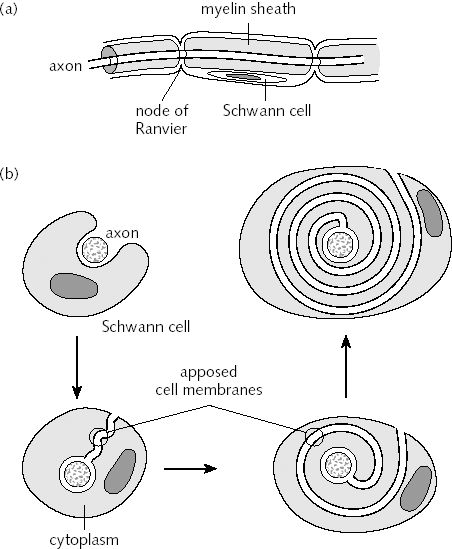
\includegraphics[height=4cm]{./images/myelin_sheath.eps}}
\caption{Myelin cell surrounding axons}\label{fig:myelin_cell}
\end{figure} 

The axon which is connected to other neurons or to the receptor is called a
{\bf transmitting axis}. 
During development, axons are guided to their appropriate targets by a variety
of guidance factors. On arriving at their synaptic targets, or while en route, axons form branches.
As with axon growth and guidance, axon branching is tightly controlled in order
to establish functional neural circuits, yet the mechanisms that
regulate this important process are less well understood.

Branching enables the axon of the neuron reaching out to targets that are not in
its direct trajectory.

\subsection{size}
\label{sec:axon-dimension}

Axonal diameters ranged from 0.15 to 1.3 $\mum$ (not including the thickness of
the myelin wrap), and tended to taper as one moved downstream.
Myelinated portions were wrapped with from 9 to 10 turns of myelin.

In axons of neurons in ventral horns of spinal cord
(Sect.\ref{sec:spinal_cord}), Pierce - Mendel (1993) found that fibers with
diameters of 0.6 $\mum$ or less were invariably unmyelinated.

% One first-order branch was also thin sectioned (diameter of 2.6 pm,
% 24 myelin turns


The axon in human neurons has the diameter of  10-20 $\mum$ and lenght of about
1 m, as it extends from the human brain to low in the spinal cord or from the
spinal cord to the fingers, etc.
{\it The longest axons are those of the sciatic nerve which run from spine to
the big toe of each foot}.

Myelinated axon conduct the electrical signal (from axon hillock -
Sect.\ref{sec:axon-hillock}) via a long distance as the signal is amplified
after a certain distance ({\it an active
process})\footnote{http://porpax.bio.miami.edu/~cmallery/150/neuro/neurophysiology.htm}.

\begin{figure}[htb]
  \centerline{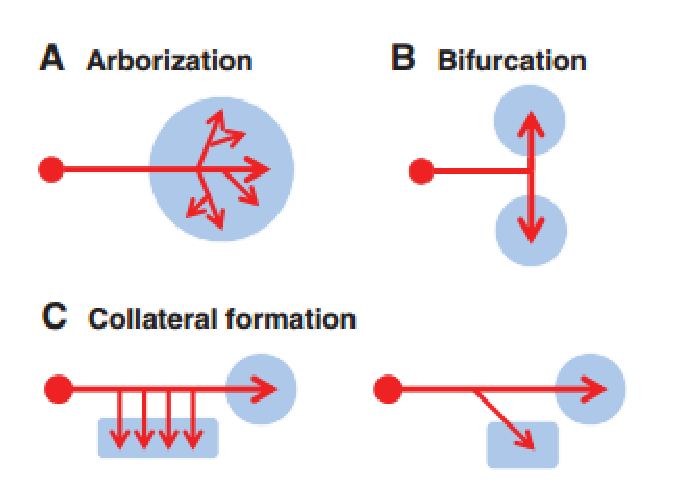
\includegraphics[height=5cm]{./images/axon_branching.eps}}
  \caption{Common axon branching processes in
  vertebrate nervous system \citep{gibson2011}}\label{fig:axon_branching}
\end{figure}

\section{Trigger zone}
\label{sec:AP-trigger-zone}
\label{sec:trigger-zone-AP}

The trigger zone is the  site of earliest firing the AP in a neuron
(Sect.\ref{sec:AP-neuron}). The {\bf trigger zone} is the site on the neurolemma
for summation of incoming graded potentials, in the forms of EPSPs and IPSPs, at
which the threshold for spiking is the lowest. Thus, the trigger zone regulates
whether or not the given neuron will initiate an action potential.

This trigger zone is considered to have a lower threshold, i.e. more excitable
than other parts of the neuron (Palay et al. (1968)) -
Fig.\ref{fig:trigger-zone}. To explain for the lower threshold of AP, there are
two common hypotheses

\begin{enumerate}
  
  \item   based on the belief that such region has high density of $\Na$
  channels  (about 20-50 times larger than in the soma or proximal dendrites).
    
  \item the mechanism for lower threshold is not the high density of $\Na$
  channel, but the shift to the left of voltage-dependency making the $\Na$
  channel more readily to open, with 7-10 more depolarized half-activation
  \citep{colbert2002}.
  
  $\beta$4 subunit of sodium channel (Sect.\ref{sec:NaR-current})
  is found enriched in AIS and nodes of Ranvier of diverse of neuronal types
  
\end{enumerate}

NOTE:
\begin{itemize}
  \item  In some neurons, the axon hillock (Sect.\ref{sec:axon-hillock}) is
  trigger zone; and less often it is the initial segment of the axon
  (Sect.\ref{sec:initial-segment-IS}).
  
  However, depending on cell types, the location of trigger zone may not be so
  closed to the soma.
  
  \item  In many other neurons, it is believed somewhere between the axon hillock
(Sect.\ref{sec:axon-hillock}) and the beginning of the myelin sheath. 
It is given the name {\bf initial segment of the axon} (or axon initial segment
AIS).
  
\end{itemize}

\begin{figure}[hbt]
 \centerline{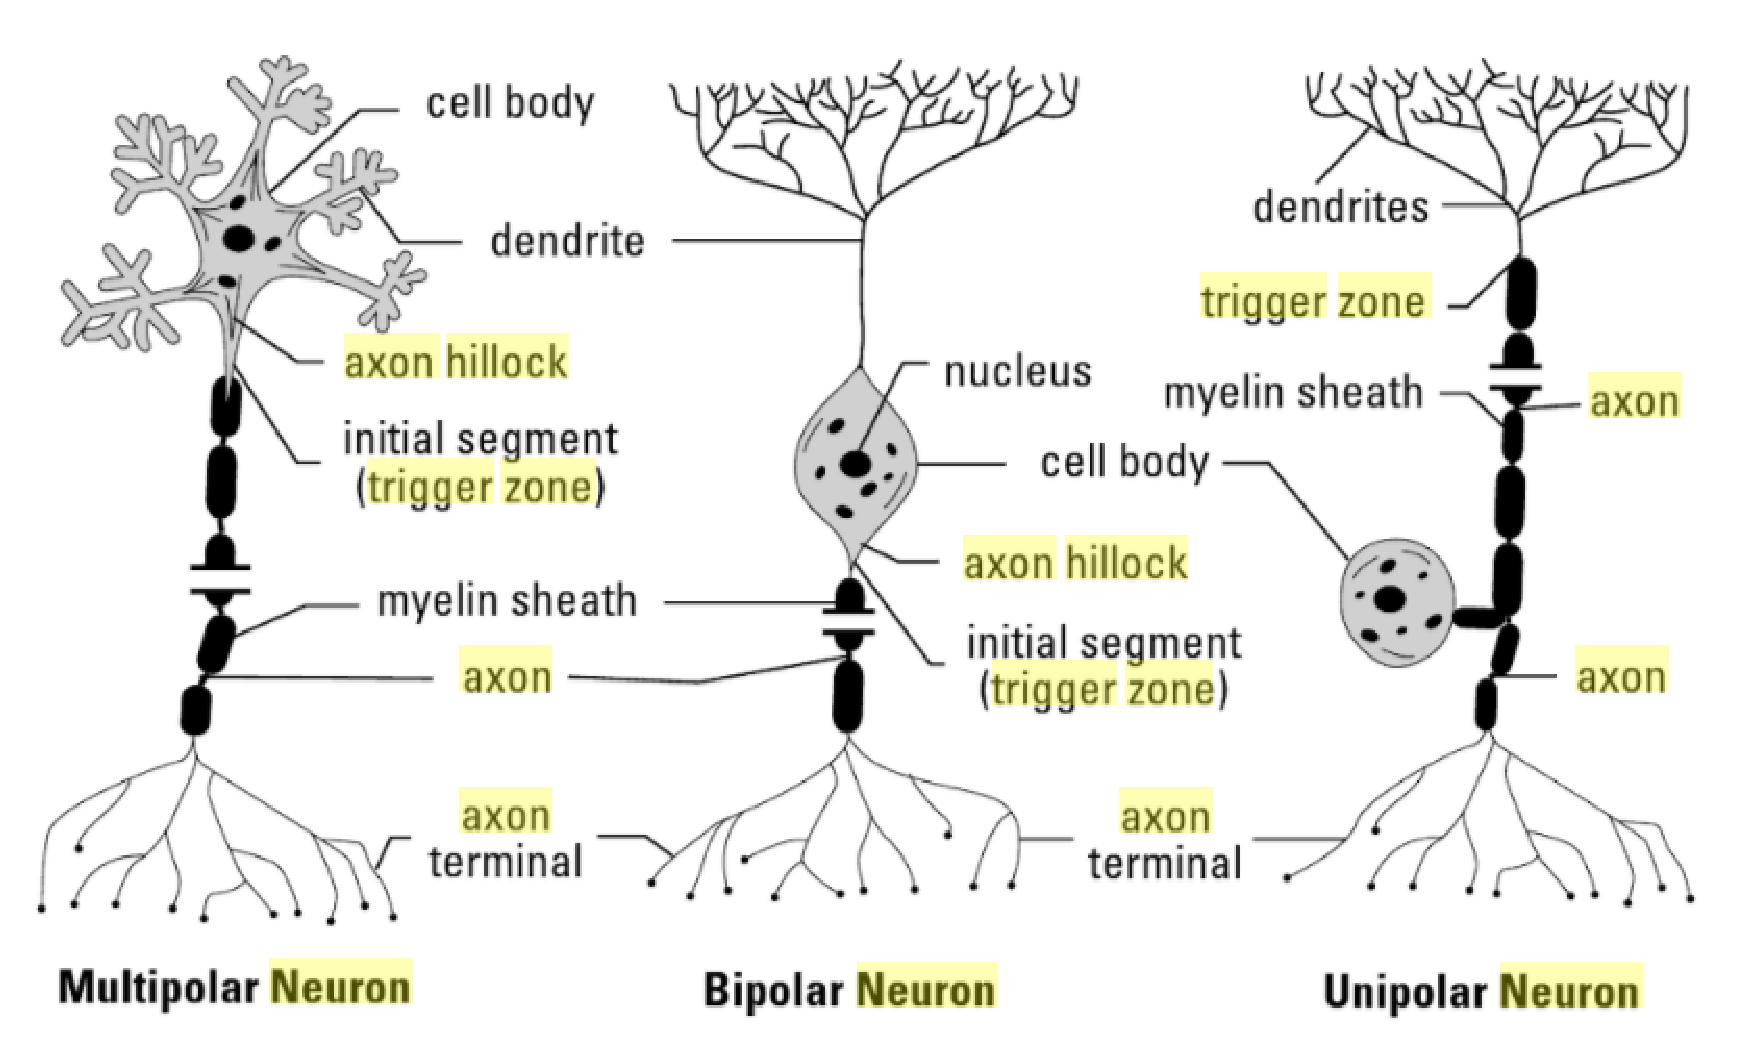
\includegraphics[height=4cm]{./images/trigger-zone.eps}}
 \caption{Trigger zone in different neuron types (reference: Steven Bassett,
 page 130 - Anatomy \& Physiology - Quick review)}
\label{fig:trigger-zone}
\end{figure}

% As the trigger zone is the place with the very high concentration of
% voltage-gated $\Na$ channels, for many years, it had been believed that the axon
% hillock was the usual site of action potential initiation. 

\section{Axon hillock}
\label{sec:axon-hillock}

The axon-hillock is a cone-shaped specialized region connecting the soma
(Sect.\ref{sec:Soma}) with the axon (Sect.\ref{sec:Axon}),
Fig.\ref{fig:hillock}. Right after that is the initial segment (IS or AIS -
Sect.\ref{sec:AIS}); even though axon hillock and IS is often treated as one,
i.e. axon hillock/initial segment (AH-IS).

Initially, it was believed that the action potential is initiated at the axon
hillock, Fig.\ref{fig:hillock}. However, recent data suggested AIS is the
trigger zone (Sect.\ref{sec:AIS}).



% \begin{figure}[hbt]
%  \centerline{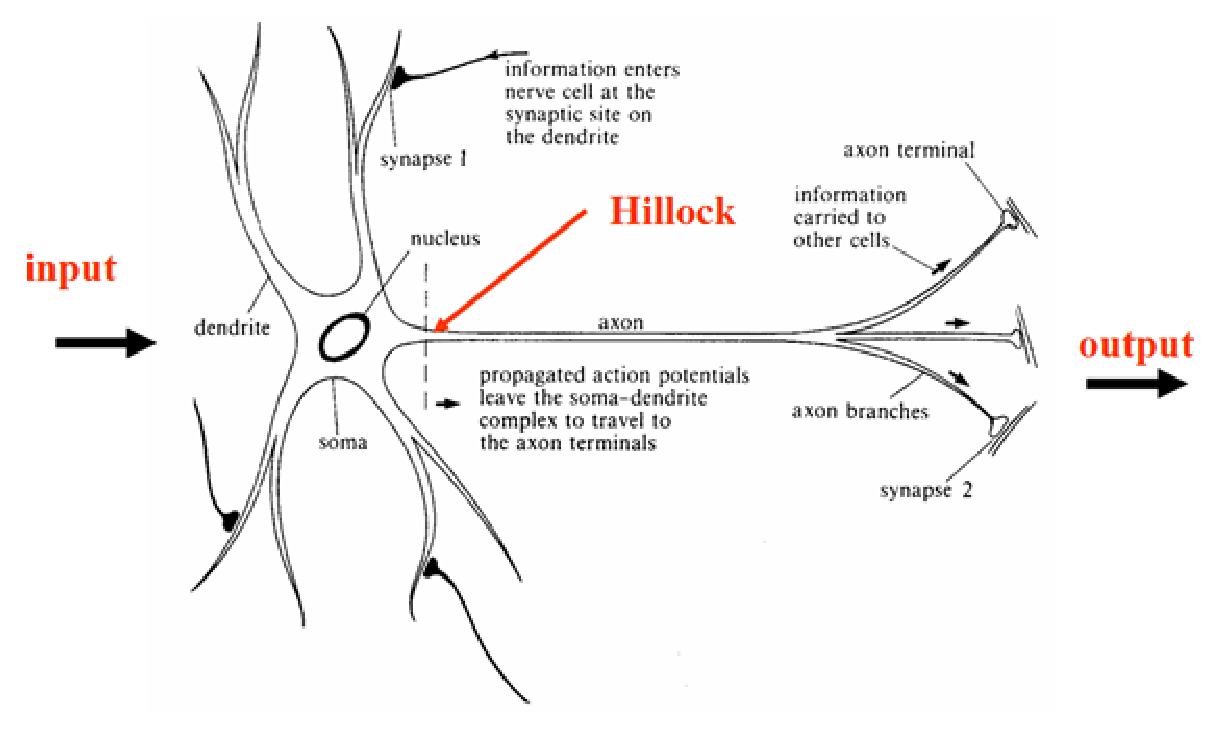
\includegraphics[height=5cm, angle=0]{./images/axon_hillock.eps}}
% \caption{Signal transmitting pathway in a nerve cell\footnote{\url{http://www.codeproject.com/KB/recipes/NeuralNetwork_1/BrainNeuron.png}}}
% \label{fig:hillock}
% \end{figure}

\begin{figure}[hbt]
 \centerline{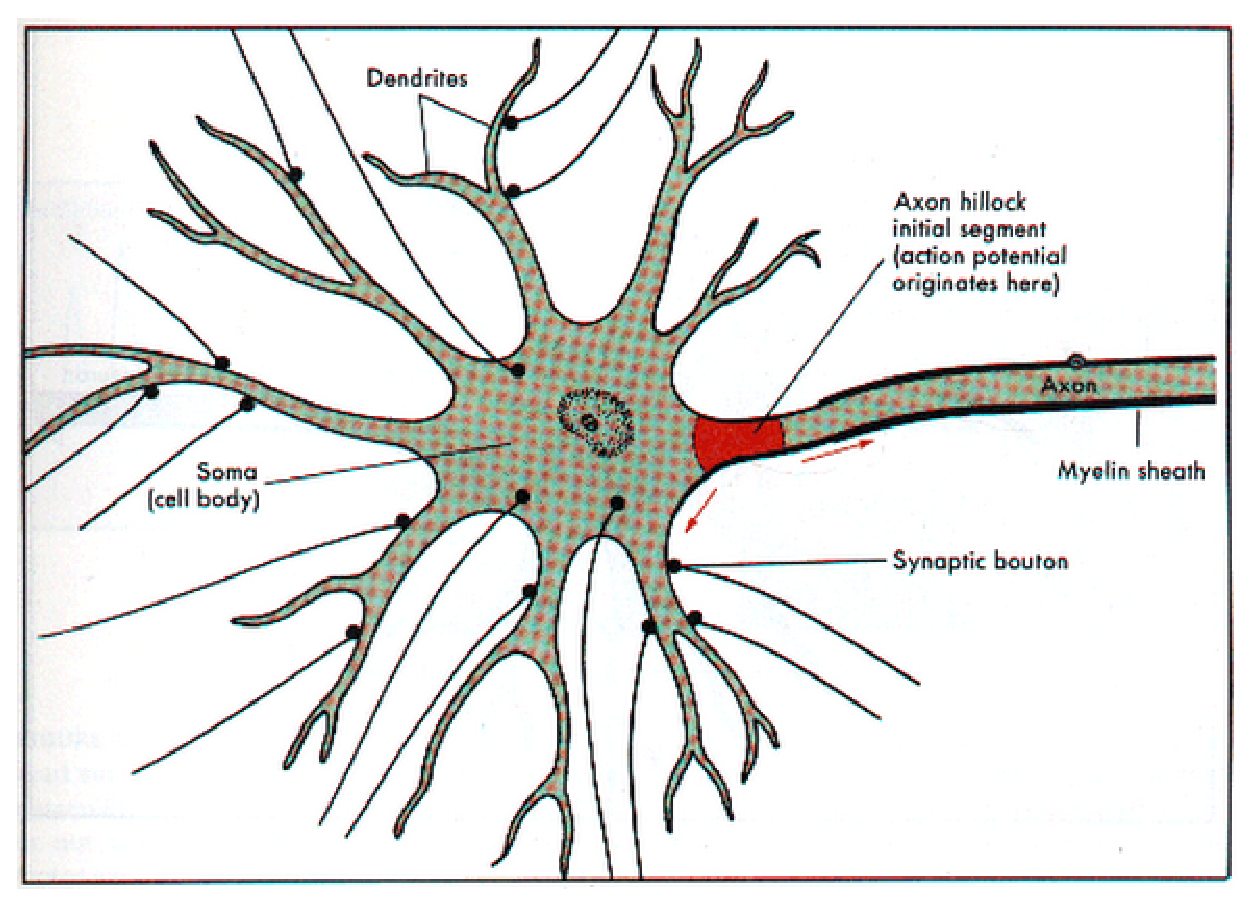
\includegraphics[height=5cm, angle=0]{./images/axon_hillock_2.eps}}
\caption{A spinal motor neuron with multiple synapse on both soma and
dendrites. The axon hillock-initial segment is the red region from which the AP
tends to originate and can propagate in two directions: along the axon or back
to the dendrite in the form called backpropagating AP which is believed to play
an important role in memory forming}
%http://www.apsubiology.org/anatomy/2010/2010_Exam_Reviews/Exam_3_Review/CH_11_Histology_of_the_Neurons_Axon.htm
\label{fig:hillock}
\end{figure}



%Thus, it requires many charges to have a significant effect on the axon
%hillock.
%\url{http://en.wikipedia.org/wiki/Axon_hillock}

\section{AIS (axon initiation segment)}
\label{sec:AIS}
\label{sec:initial-segment-IS}
\label{sec:axon-initial-segment-AIS}


Excitatory and inhibitory synaptic inputs are integrated at the axon initial
segment (AIS). The AIS is a proximal part of the axon about 40 $\mum$ in length,
right after the axon hillock (Sect.\ref{sec:axon-hillock}). The location of AIS
vary from neuron to neuron. In pyramidal neurons, it is typically enclosed by
two points: from the distance 35$\mum$ to the soma to 50$\mum$ to the soma, upto
the onset of myelination. The onset of myelination is typically 50$\mum$ from
the soma in cortical pyramidal L5 neurons.

Indeed, the earliest site of action potential initiation is found just adjacent,
in the initial (unmyelinated) segment of the axon (Sect.\ref{sec:AIS})
\citep{clark2009}. However, the positive point, at which the action potential
starts, varies between cells. This location can also be altered by hormonal
stimulation of the neuron, or by second messenger effects of neurotransmitters.
If it pass the threshold, then an AP is initiated and being transmitted to the
axon, and/or as the backpropagating AP (Sect.\ref{sec:back-propagating_AP}).

\begin{itemize}
  
  \item  in pyramidal neuron (Sect.\ref{sec:pyramidal-neurons}): it is at a
 location typically 30-50 $\mum$ from the cell body, which is far enough from
 the cell body making the recorded AP in the cell body with non-uniformity of voltage.
   
% So, we can generally say the initiation site is axon hillock-initial segment.
% 
% \footnote{\url{http://en.wikipedia.org/wiki/Axon_hillock}}

 
\end{itemize}

The AIS is characterized by the fasciculation of microtubules, and is
believed as the trigger zone  (Sect.\ref{sec:AP-trigger-zone}). 


Most of the studies on AIS have focused on excitatory cells, in which the action
potential initiation site is located in the distal region of the AIS.
Interestingly, the AIS contains specialized subdomains; the distal part is
enriched in NaV1.6 (Sect.\ref{sec:Nav1.6}), whereas the proximal part is
enriched in Nav1.2 (Sect.\ref{sec:Nav1.2}).
A recent study has shown that NaV1.6 channels in the distal AIS promote action
potential initiation, whereas NaV1.2 channels in the proximal AIS promote its
backpropagation to the soma - Hu et al. (2009)
%Hu W, Tian C, Li T, Yang M, Hou H, Shu Y. Distinct contributions of Na(v)1.6
% and Na(v)1.2 in action potential initiation and backpropagation. Nat Neurosci. 2009;12:996-1002. 

Similar to neurons with myelinated axons, the AIS is also the site of action
potential initiation in unmyelinated glutamatergic neurons, which contains
Nav1.2 and, to a lesser extent, Nav1.6 channels.
However, in these neurons the AIS lacks the structural and morphological
characteristics of that of myelinated axons, and action potentials are usually initiated in the proximal part.
\url{http://www.ncbi.nlm.nih.gov/books/NBK98195/}

Recent studies have shown that Nav1.1 is particularly important for the
excitability of GABAergic neurons (58, 59; see Nicotinic acetylcholine receptor
mutations), and these channels are clustered at the AIS of some types of
interneurons, including parvalbumin-positive, fast-spiking interneurons.

\section{Axon branching: arborization, collateral, bifurcation}

The axon ends with many (sometimes up to 10,000) end-branches terminals
\footnote{\url{http://www.fortunecity.com/greenfield/buzzard/387/nervecellgen.htm}},
known as {\it telodendria} (Greek: = tree + end) (Sect.\ref{sec:telodendria}).
As shown in the Fig.\ref{fig:neuron_cell}, branching in neuron can be very
extensive which makes axon terminal to be very small.
In the case of Purkinje fibre, the surface area of dendritic tree can be as much
as  80-100 that of the soma. In the case of pyramidal cells or motoneurons, the
dendritic surface area is of about 10-20 times that of the soma.

Axonal branches appear in different shapes, form at different
locations, and change with time. 
\textcolor{red}{Note that the axon grows, i.e. extension, from the growth cone}.
Axon branching can be classified into 3 forms:
\citep{gibson2011}
\begin{enumerate}
  \item {\bf bifurcation} (simplest shape): Bifurcation of the growth
  cone at the tip of the axon during axon extension, i.e. generating
  two daughter branches. This mode is ideal for generating Y-shaped or T-shaped
  axon branches. 
  
  Example: found in central sensory projections into the spinal cord.
  
  This is however, not a major mechanism of axon branching.
  It is suspected that bifurcation-mediated branching may be an inherent
  response of growth cones when they encounter an environment
that does not allow them to advance, and the growth cone splits sending two
different growth cones to scout additional routes. \citep{gallo2011}

  \item {\bf collateral branches} (\textcolor{red}{This is the major
  mechanism}):
  The main axon (axon shaft) gives off occasional branches, at location behind the growth cone, called {\bf axon
  collaterals}.   This typically occurs at location far from the axon terminal.
  
The generation of axon collateral branches allows individual neurons to make
contacts with multiple neurons within a target and with multiple targets.
  
  \item {\bf arborization}: This typically occurs at
  the axon terminal, forming the tree-like arbors with high-order branches. 
  
  Example: found in ganglion cells (Sect.\ref{sec:ganglion})
  and sensory neurons (Sect.\ref{sec:sensory_neuron}). 

\end{enumerate}
Arborization or Bifurcation branching to occur depends on the presence of
branch-promoting factors at the axon terminal such as nerve growth factor (NGF),
wingless-related MMTV integration site (Wnt) factors and C-type natriuretic
peptide (CNP). 

Colleteral branching occurs at a middle region of the axon (not at the terminal)
depends on the presence of a positive branch-promoting cue or by a mechanism
involving local inhibition \citep{gibson2011}.
\citep{gallo2011} showed that there are three methods of axon collateral branching
\begin{enumerate}
  \item filopodial method
  
  \item lamellipodial method
  
  \item growth cone pausing method: 
  here, the mechanism of axon extension and branching are not the same.
\end{enumerate}

%Axon's length is up to several feet in length. 



\section{Telodendria}
\label{sec:telodendria}

The axon (Sect.\ref{sec:Axon}) has many end-branch terminal called {\bf
telodendria}.  As the axon propagate the signal, when it reaches these ends, the
signal needs a mechanism to be transmitted to the other nervel cells.
At the end of the telodendria is the foot-like axon terminals which form a
junction called {\bf synapse} with another neurons.


\section{Apical tuft}
\label{sec:apical-tuft}

The apical tuft is the most remote area of the dendritic tree of neocortical
pyramidal neurons. Despite its distal location, the apical dendritic tuft of
layer 5 pyramidal neurons receives substantial excitatory synaptic drive and
actively processes corticocortical input during behavior


\section{Actin remodeling}
\label{sec:actin_remodeling}

Actin remodeling of neurons refers to the process to change the shape and
structure of dendritic spines (Sect.\ref{sec:dendritic_spines}) due to the
protein actin.

There are two types of protein actin
\begin{itemize}
  \item {\bf G-actin} is the monomer form of actin, and is uniformly distributed
  throughout axon and dendrite
  \item {\bf F-actin} is the polymer form of actin, and is presence in the
  dendritic spines.
\end{itemize}
Because the actin cytoskeleton is so big, it can easily change cell morphology
just by assembling or disassembling itself.
\url{http://www.ncbi.nlm.nih.gov/books/NBK21493/}

Actin remodeling consists of the dynamic changes in F-actin that
underlie the morphological changes at the neural synapse.
The formation of F-actin promotes long-term potentiation (LTP -
Sect.\ref{sec:LTplasticity}); otherwise, when F-actin is unabled to form,
long-term depression (LTD) is induced, Fig.\ref{fig:F-actin_and_LTP-LTD}.
\begin{itemize}
  \item LTP environment causes larger spine volume, increased cell
  communication, and a greater ratio of F-actin to G-actin.
  
  \item LTD environment, spine volume is decreased, cell communication is
  decreased, and there is a far greater ratio of G-actin to F-actin.
\end{itemize}

\begin{figure}[htb]
  \centerline{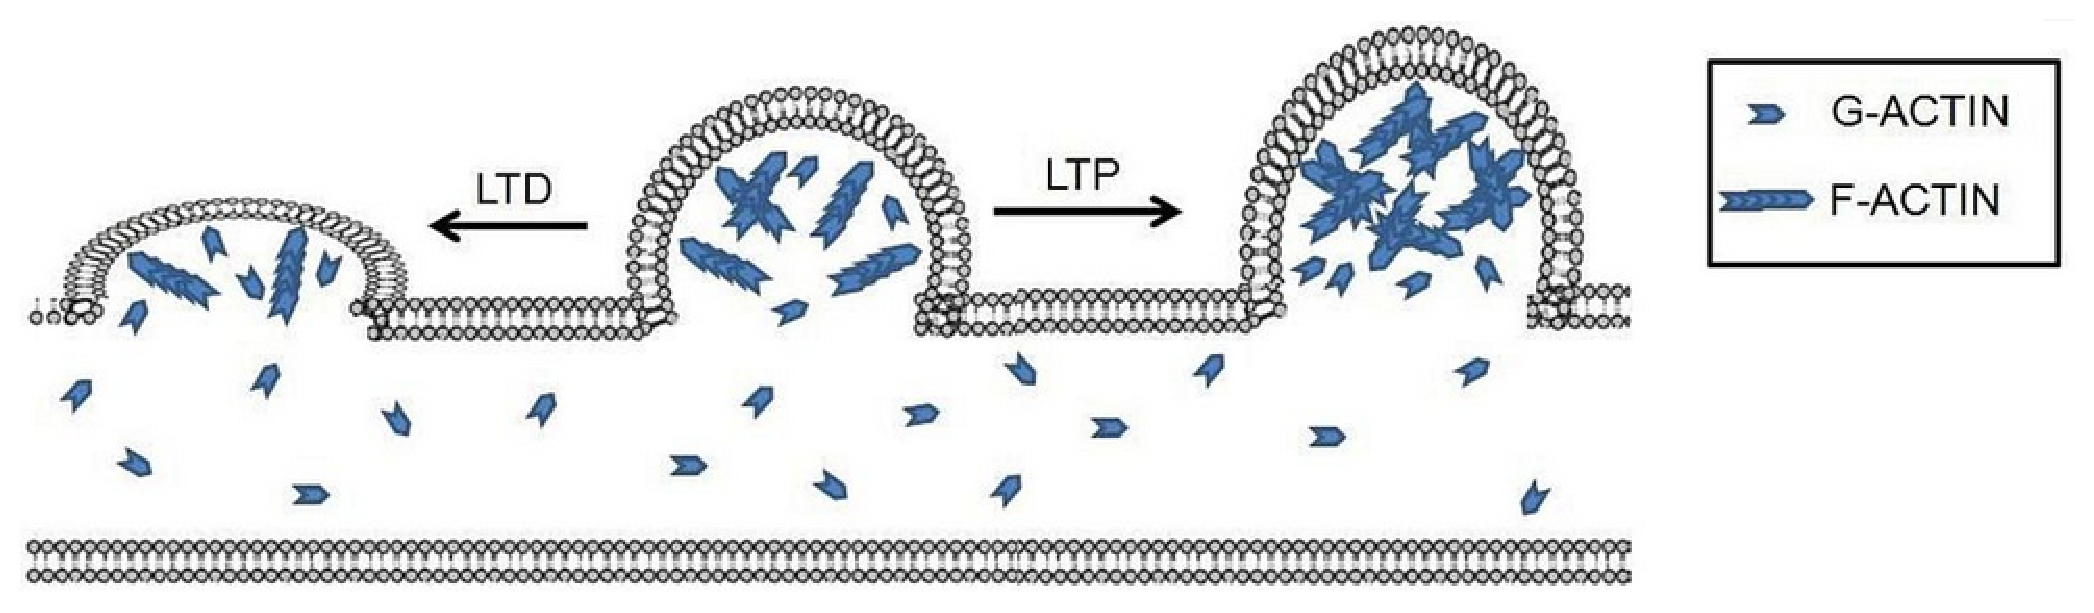
\includegraphics[height=3cm]{./images/F-actin_and_LTP-LTD.eps}}
  \caption{Morphological effects on the dendrites in LTP and LTD
  environments based on F-actin/G-actin ratio}
%http://en.wikipedia.org/wiki/Actin_remodeling_of_neurons  
\label{fig:F-actin_and_LTP-LTD}
\end{figure}

At presynaptic region, actin allows the formation of new axonal branches
(new boutons), and facilittes the formation of recruitment of vesicles to the
boutons.

At postsynaptic region (e.g. dendritic spines), actin controls the
formation of new spines, increase/decrease in volume. 

We need to consider these factors in controlling actin
\begin{itemize}
  \item synaptopodin: (at postsynaptic dendrite and dendritic spines)
  actin-associated protein that may play a role in actin-based cell shape and
  motility.
  \url{http://en.wikipedia.org/wiki/SYNPO}
  
  \item actin regulators: small GTPases such as Rac, RhoA, and CDC42
  
\end{itemize}
 

\section{Some numbers and facts}
\label{sec:some-numbers}

Here are some numbers and facts
\begin{itemize}
\item About $10^{12}$ neurons in human brain.
\item A typical $1$ mm$^3$ cortical tissue contain $10^5$ neurons. 
\item Neuron has very diverse shape (morphological), about 10,000 in
  vertebrate brain
\item The number of functionally different classes of neurons is even
  higher, as neuron of the same morphology can have different
  functions, e.g those of pyramidal cells. 
\item There are about $10^{15}$ synapses in human brain
\item Synapse can be either electrical (allow current flow) or
  chemical (allow neurotransmitter to across). Electrical synapses
  often have specialized proteins that form ionic channels bridging
  the interior of two neurons and allow the current from one neuron to
  flow to the other. 
\item Number of synapse for a single neuron may vary, e.g. motor
  neuron has about $10^4$ synapse. 
\item Synapses do not always unidirection, i.e. reciprocal synapse
  (feedback on the previous neuron), serial synapse (form local loop),
  lateral synapse (with parallel neuron). 
\end{itemize}

